\documentclass[compress,10pt]{beamer}
% version imprimable pour assistance
%\documentclass[10pt, green, handout]{beamer}
\usepackage[T1]{fontenc}
\usepackage[utf8]{inputenc}
\usepackage[frenchb]{babel} % le document est en français
\usepackage{rotating,amsmath}
\usepackage{graphicx,cancel}       % pour ins\'erer des figures
        % pour d\'efinir plus de couleurs
\usetheme{Malmoe}  %Applique le theme INRA (ce dernier doit être present dans le repertoire courant)
\usepackage{xcolor,colortbl}
\usepackage{array}
\usepackage{mdframed}
\usepackage{listings}
\usepackage{lmodern}	
\usepackage{tikz}
\usetikzlibrary{positioning,shapes,arrows}


\definecolor{lgreen}{RGB}{188,214,49}
\definecolor{dgreen}{RGB}{139,172,33}
%\setbeamercolor{structure}{fg=INRA@dinst}

\setbeamertemplate{blocks}[rounded][shadow=true]
\setbeamercolor{block title}{use = structure , fg=dgreen, bg = dgreen!35}
\setbeamercolor{normal text}{fg=black,bg=white}
\setbeamercolor{alerted text}{fg=lgreen}
\setbeamercolor{example text}{fg=lgreen}
\setbeamercolor{structure}{fg=dgreen} %d'où ce bleu par défaut
\setbeamercolor{background canvas}{parent=normal text}


 \usepackage{tikz}

\usetikzlibrary{calc,shapes,backgrounds,arrows,automata,shadows,positioning}



\addtobeamertemplate{navigation symbols}{}{%
    \usebeamerfont{footline}%
    \usebeamercolor[fg]{footline}%
    \hspace{1em}%
    \insertframenumber/\inserttotalframenumber
}



\setbeamertemplate{frametitlecontinuation}{\insertcontinuationcountroman}

%-------------------------------------------------------------------------------
% Quelques options pdf
%-------------------------------------------------------------------------------
\hypersetup{
pdfpagemode = FullScreen, % afficher le pdf en plein \'ecran
pdfauthor   = {},%
pdftitle    = {},%
pdfsubject  = {},%
pdfkeywords = {Science,Impact},%
pdfcreator  = {PDFLaTeX,emacs,AucTeX},%
pdfproducer = {INRA}%
}


\newcommand\Wider[2][3em]{%
\makebox[\linewidth][c]{%
  \begin{minipage}{\dimexpr\textwidth+#1\relax}
  \raggedright#2
  \end{minipage}%
  }%
}

\AtBeginSection[]
{  \begin{frame}
  \frametitle{}
  \tableofcontents[currentsection, hideothersubsections]
  \end{frame} 
}



%
\newcommand{\bX}{\boldsymbol{X}}

\newcommand{\Xall}{\bX}
\newcommand{\Zall}{\bZ}
\newcommand{\M}{\mathcal{M}_{K_0,K_1,\dots, K_Q}}
\newcommand{\ind}{\mathds{1}}

\newcommand{\Mcal}{\mathcal{M}}


\newcommand{\bZ}{\boldsymbol{Z}}
\newcommand{\bpi}{\boldsymbol{\pi}}
\newcommand{\balpha}{\boldsymbol{\alpha}}
\newcommand{\btau}{\boldsymbol{\tau}}


\def\Ecal{\mathcal{E}}



\def\N{\mathbb{N}}
\def\R{\mathbb{R}}
\def\F{\mathcal{F}}
\def\Nb{\boldsymbol{N}}
\def\bZ{\boldsymbol{Z}}
\def\btheta{\boldsymbol{\theta}}
\def\bpi{\boldsymbol{\pi}}
\def\bY{\boldsymbol{Y}}
\def \ind{\mathbb{I}}
\def \P{\mathbb{P}}
\def \vert{\color{dgreen}}

\def \rouge{\color{red}}
\def \noir{\color{black}}
%-------------------------------------------------------------------------------
\title[Formation Réseaux 06/2019]{ Données de réseaux : modèles probabilistes }
%\subtitle{}
\author[Donnet, Massol, Verzelen]{ Sophie Donnet, François Massol, Nicolas Verzelen\\ MIA Paris, INRA}
\titlegraphic{
\includegraphics[width=2cm]{plots/logoINRA.png}
}
\date{Formation Réseaux MIRES / ReSodiv/ CoEx\\ 18-19-06/2019}
%-------------------------------------------------------------------------------
\begin{document}

%-F1------------------------------------------------------------------------------
\begin{frame}
\titlepage
\end{frame}

\setbeamertemplate{background canvas}[default]

%------------------------------------------------------------

%----------------------------------------------------------------------------------- 

\begin{frame}{Qu'attendre des SBM? }
 Outils automatiques pour faire des groupes de sommets qui ont le même rôle dans le réseau 
 
\begin{overlayarea}{10cm}{20cm}

\only<1>{ \begin{tabular}{cc}
  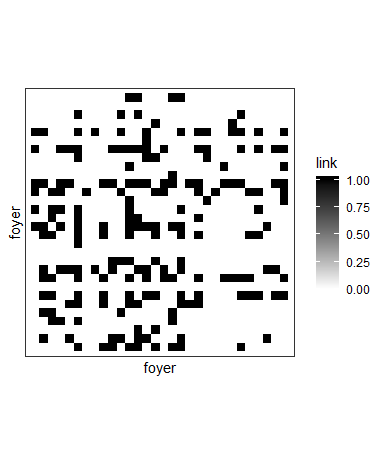
\includegraphics[width = 5cm]{plots/Vanuatu_matrix.png} &
 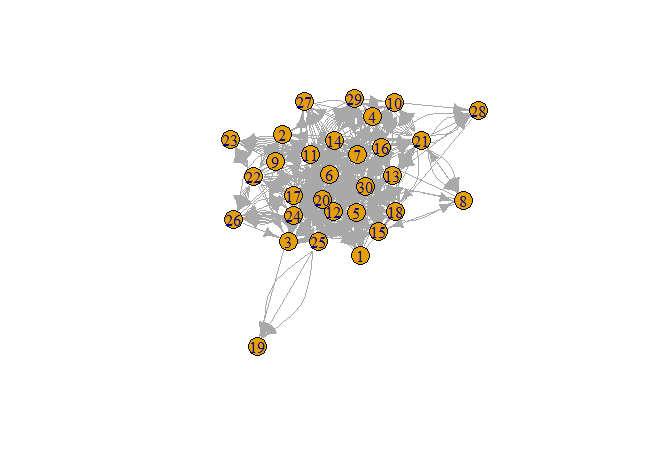
\includegraphics[width = 5cm]{plots/Vanuatu_directed.png}
\end{tabular}}


\only<2>{ \begin{tabular}{cc} 
  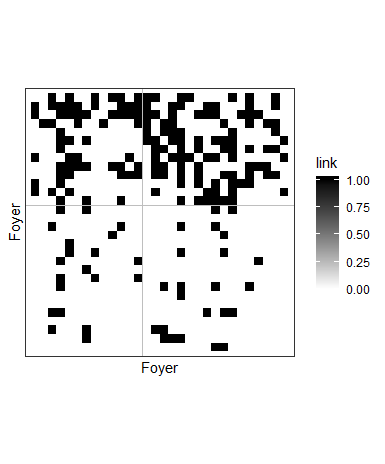
\includegraphics[width = 5cm]{plots/Vanuatu_estimmatrix.png} &
 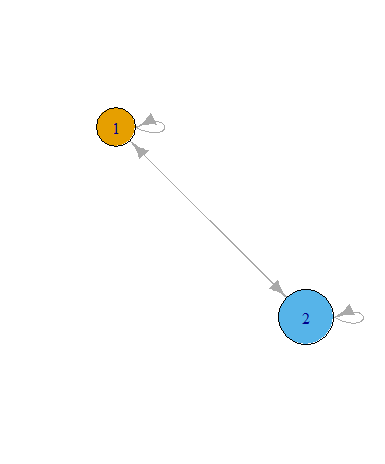
\includegraphics[width = 5cm]{plots/Vanuatu_graphestim.png}
\end{tabular}
}

\end{overlayarea}


\end{frame}



%-------------------------------------------------------------------------------

\begin{frame}{A propos de l'aspect ``probabiliste''}

\begin{itemize}
\item \emph{Hypothèse}: réseau observé $y_{ij}$ réalisation d'un phénomène aléatoire
\item \emph{Modèle}:  forme particulière de ce phénomène
\item \emph{Aléa} :  représente le fait que l'observateur n'est pas capable de prédire $y_{ij}$

\begin{itemize}
\item Exemple de l'expérience du Pile ou Face
\item  Si je connaissais tous les paramètres physiques de la pièce et du lancer, je serais capable de prédire l'issue du jeu
\item En tant qu'observateur, je ne peux pas prédire : expérience aléatoire
\end{itemize}

\end{itemize}

\end{frame}

%-------------------------------------------------------------------------------



%--------------------


\begin{frame}
\frametitle{A first random graph model for network: null model}

\begin{itemize}
\item  \textcolor{blue}{Erd\H{o}s-Rényi (1959)} Model for $n$ nodes 
\item 

Let $(y_{ij})_{i,j  = 1\dots n}$ be an adjacency matrix (i.e. representing a simple network) with $y_{ij}\in \{0,1\}$ 

\item 
ER assumes that $y_{ij}$ is the realisation of :

$$\forall 1\le i,j\le n,\quad Y_{ij}\overset{i.i.d.}{\sim} Bern(p),$$
where $Bern$ is the Bernoulli distribution and $p\in[0,1]$ a probability for a link to exist. 
\end{itemize}
\end{frame}

\begin{frame}
\frametitle{A first random graph model for network: null model}

\begin{center}
 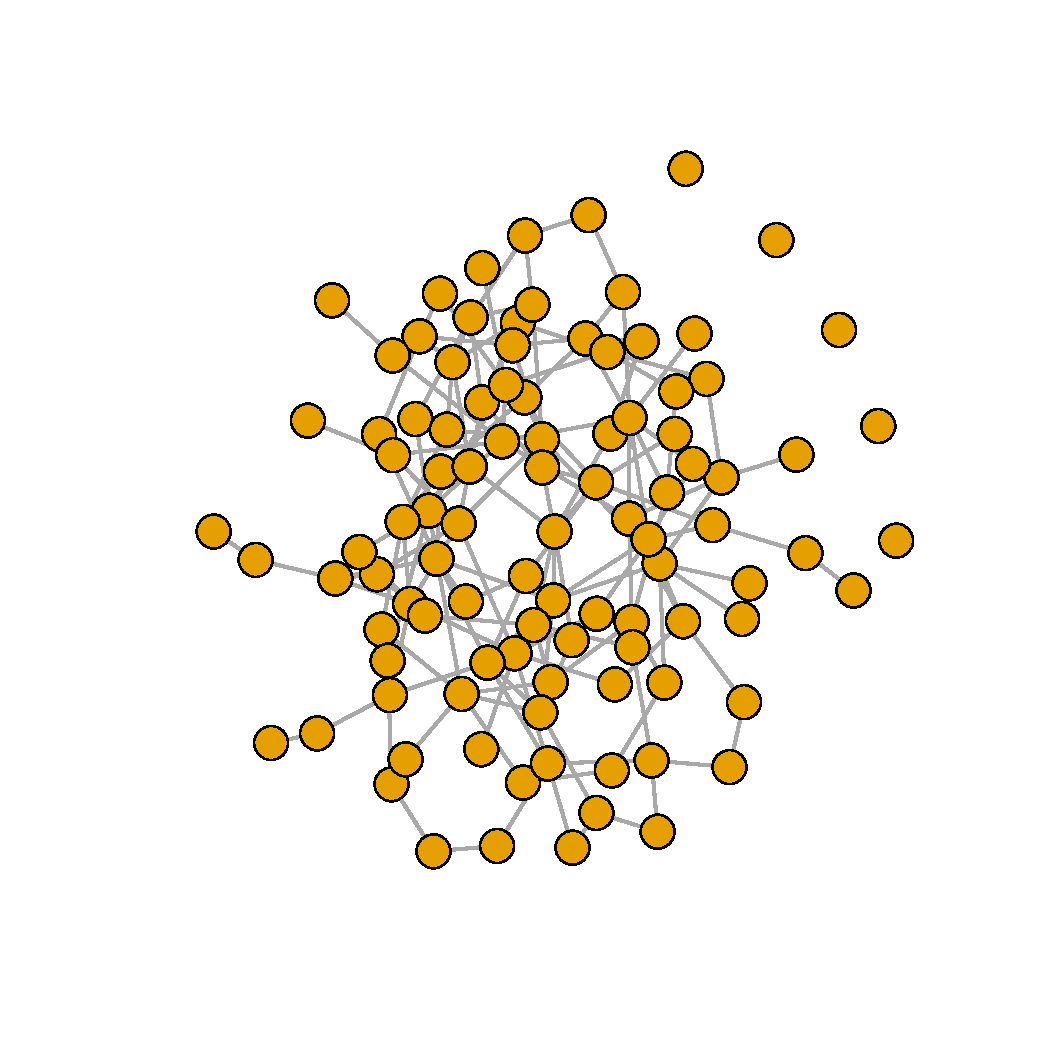
\includegraphics[scale=.3]{plots/ER.pdf} 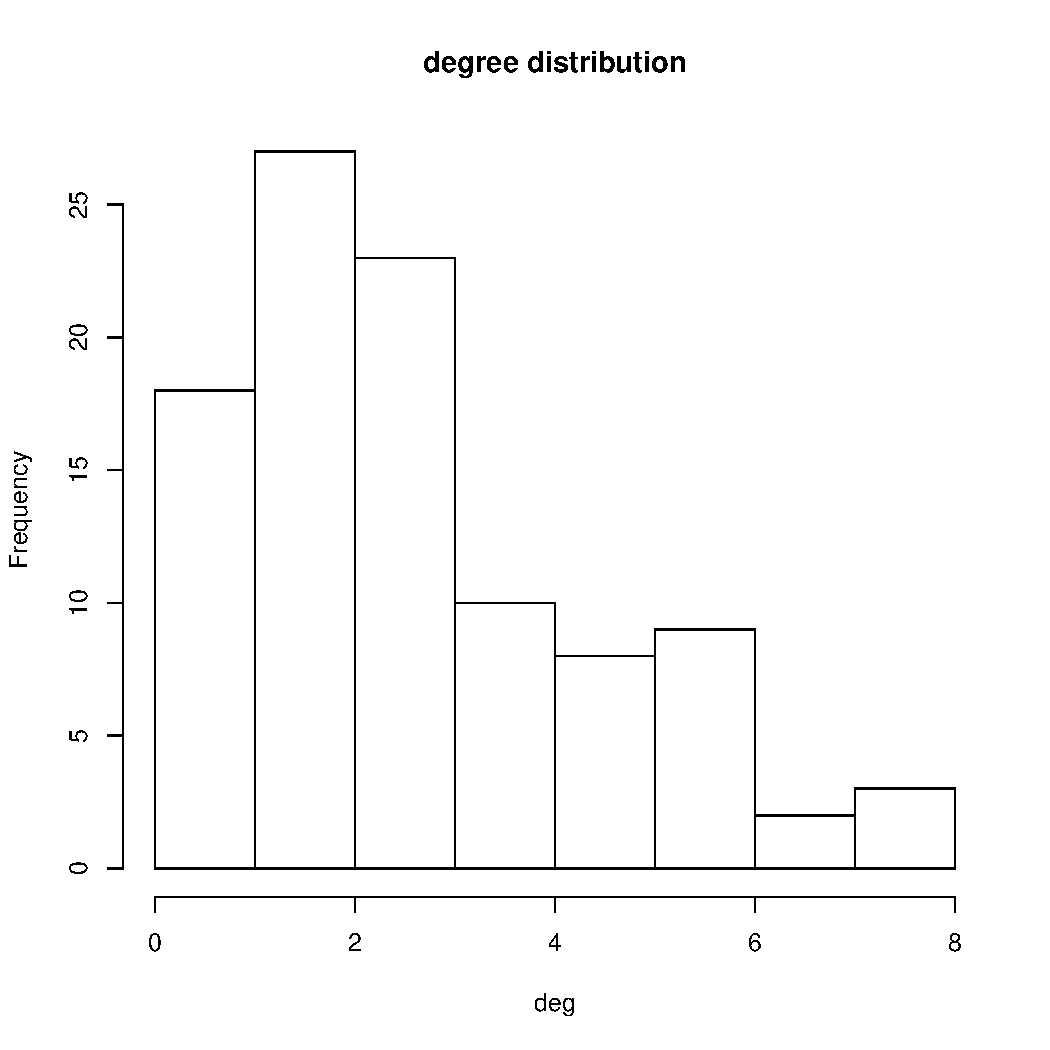
\includegraphics[scale=.3]{plots/degER.pdf}
\end{center}


\textbf{\textcolor{dgreen}{Limitations of an ER graph to describe real networks}}
\begin{itemize}
 \item Degree distribution too concentrated, no high degree nodes,
 \item All nodes are equivalent (no nestedness...),
 \item No modularity.

 \end{itemize}
 

\end{frame}

%-------------------------------------------------------------------------------------



%-------------------------------------------------------------------------------------
\section{Stochastic Block Model (SBM)}
%-----------------------------------------------------------------

\begin{frame}  \frametitle{Stochastic Block Model}

\textcolor{blue}{Nowicki, \& Snijders (2001)}

Let ($y_{ij}$) be an adjacency matrix such that $y_{ij} \in \{0,1\}$.  $y_{ij}$ is the realisation of the following processus. 

\begin{block}{Latent variables}
\begin{itemize}
\item The nodes $i= 1,\dots,n$ are partitionned into $K$ clusters
\item $Z_i = k$ if node $i$ belongs to cluster (block) $k$
\item $Z_i$ independant variables
$$ \mathbb{P}(Z_i = k) = \pi_k$$
\end{itemize}
\end{block}

\begin{block}{Conditionally to $(Z_i)_{i=1,\dots,n}$... }

$(Y_{ij})$ independant and 
\begin{eqnarray*}
 Y_{ij}  | Z_i, Z_j \sim  \mathcal{B}ern(\alpha_{Z_i,Z_j}) \quad \Leftrightarrow \quad  P(Y_{ij} = 1 | Z_i = k, Z_j = \ell)  =  \alpha_{k\ell}
\end{eqnarray*}
\end{block}
 


\end{frame}


%-------------------------------------------------------------------------------------

\begin{frame}
  \frametitle{Stochastic Block Model : illustration}

  \begin{center}
    \begin{overlayarea}{\textwidth}{.5\textheight}
      \begin{columns}
        \begin{column}{.45\paperwidth}
        \begin{tikzpicture}
          %% UN GRAPH

          \tikzstyle{every edge}=[-,>=stealth',shorten >=1pt,auto,thin,draw]
          \tikzstyle{every state}=[draw=none,text=white,scale=0.65, font=\scriptsize, transform shape]
          \tikzstyle{every node}=[fill=yellow!40!orange]
          % premier cluster
          \node[state] (A1) at (0,0.5) {A1};
          \node[state] (A2) at (1,0.5) {A2};
          \node[state] (A3) at (.5,1.5) {A3};

          \path (A2) edge [bend left] node[fill=white,below=.1cm]
          {$\alpha_{\textcolor{yellow!40!orange}{\bullet}\textcolor{yellow!40!orange}{\bullet}}$}
          (A1)
          (A1) edge [bend left] (A3)
          (A3) edge [bend left] (A2);

          \tikzstyle{every node}=[fill=blue!80!black]
          \foreach \angle/\text in {234/B1, 162/B2, 90/B3, 18/B4, -54/B5} {
            \node[fill=blue,state,xshift=5cm,yshift=3.5cm]     (\text)    at
            (\angle:1cm) {\text};
          }
          \path (B2) edge (B5)
          (B1) edge (B4);
          \foreach \from/\to in {1/2,2/3,4/5,5/1}{
            \path (B\from) edge [bend left] (B\to);
          }

          \path    (B3)    edge     [bend    left]    node[fill=white]
          {$\alpha_{\textcolor{blue!80!black}{\bullet}\textcolor{blue!80!black}{\bullet}}$}  (B4) ;
          
          \tikzstyle{every node}=[fill=green!50!black]
          % troisieme cluster
          \node[state] (C1) at (3,-.5) {C1};
          \node[state] (C2) at (4,0) {C2};

          \path (C1) edge [bend right] node[fill=white,below=.25cm]
          {$\alpha_{\textcolor{green!50!black}{\bullet}\textcolor{green!50!black}{\bullet}}$}
          (C2);

          % inter cluster
          \path (A3) edge [bend right]  (B2)
          (A3)    edge    [bend    left]    node[fill=white]
          {$\alpha_{\textcolor{yellow!40!orange}{\bullet}\textcolor{blue!80!black}{\bullet}}$}
          (B3)
          (C2) edge [bend right] node[fill=white,right]
          {$\alpha_{\textcolor{blue!80!black}{\bullet}\textcolor{green!50!black}{\bullet}}$}
          (B4)
          (A2) edge [bend right] node[fill=white]
          {$\alpha_{\textcolor{yellow!40!orange}{\bullet}\textcolor{green!50!black}{\bullet}}$}
          (C1);
        \end{tikzpicture}
        \end{column}


        \begin{column}{.5\paperwidth}
          \begin{small}
            \begin{block}{Parameters}
              Let $n$ nodes divided into $3$ clusters
              \begin{itemize}
              \item
                $\mathcal{K}=\{\textcolor{yellow!40!orange}{\bullet},\textcolor{blue!80!black}{\bullet},\textcolor{green!50!black}{\bullet}\}$
                 clusters
              \item  $\pi_\bullet  =  \mathbb{P}(i  \in  \bullet)$,
                $\bullet\in\mathcal{K},i=1,\dots,n$
              \item      $\alpha_{\textcolor{yellow!40!orange}{\bullet}\textcolor{blue!80!black}{\bullet}}     =      \mathbb{P}(i
                \leftrightarrow j | i\in\textcolor{yellow!40!orange}{\bullet},j\in\textcolor{blue!80!black}{\bullet})$
              \end{itemize}
            \end{block}
          \end{small}
        \end{column}
      \end{columns}
    \end{overlayarea}
  \end{center}
  
%\begin{eqnarray*}
%&(Z_i) &  \ \sim^{\text{iid}} \mathcal{M}(1,\alpha) \ \text{et} \  Z_{i} \in \{1,...,Q\}, \\ 
% &(Y_{ij})&| \ \{Z_{i},Z_{j}\} \sim^{\text{ind}} \mathcal{B}(\pi_{Z_{i}Z_{j}}).\\
%\end{eqnarray*}

% Proposition Julien
\begin{align*}
Z_i = \mathbf{1}_{\{i \in \bullet\}}  \ & \sim^{\text{iid}} \mathcal{M}(1,\pi), \quad \forall\bullet \in \mathcal{K}, \\ 
Y_{ij} \ | \ \{i\in\textcolor{yellow!40!orange}{\bullet},j\in\textcolor{blue!80!black}{\bullet}\}
& \sim^{\text{ind}} \mathcal{B}(\alpha_{\textcolor{yellow!40!orange}{\bullet}\textcolor{blue!80!black}{\bullet}})\\
\end{align*}

\end{frame}


%-------------------------------------------------------------------------------------


\begin{frame}
\frametitle{SBM : A great generative model}

\begin{itemize}
\item  Generative model : easy to simulate
\item No a priori on the type of structure
\item Combination of modularity, nestedness, etc... 
\end{itemize}
\end{frame}

%-------------------------------------------------------------------------------------

\begin{frame}
\frametitle{Networks with hubs generated by SBM}

\centering
\begin{tabular}{ccc}
 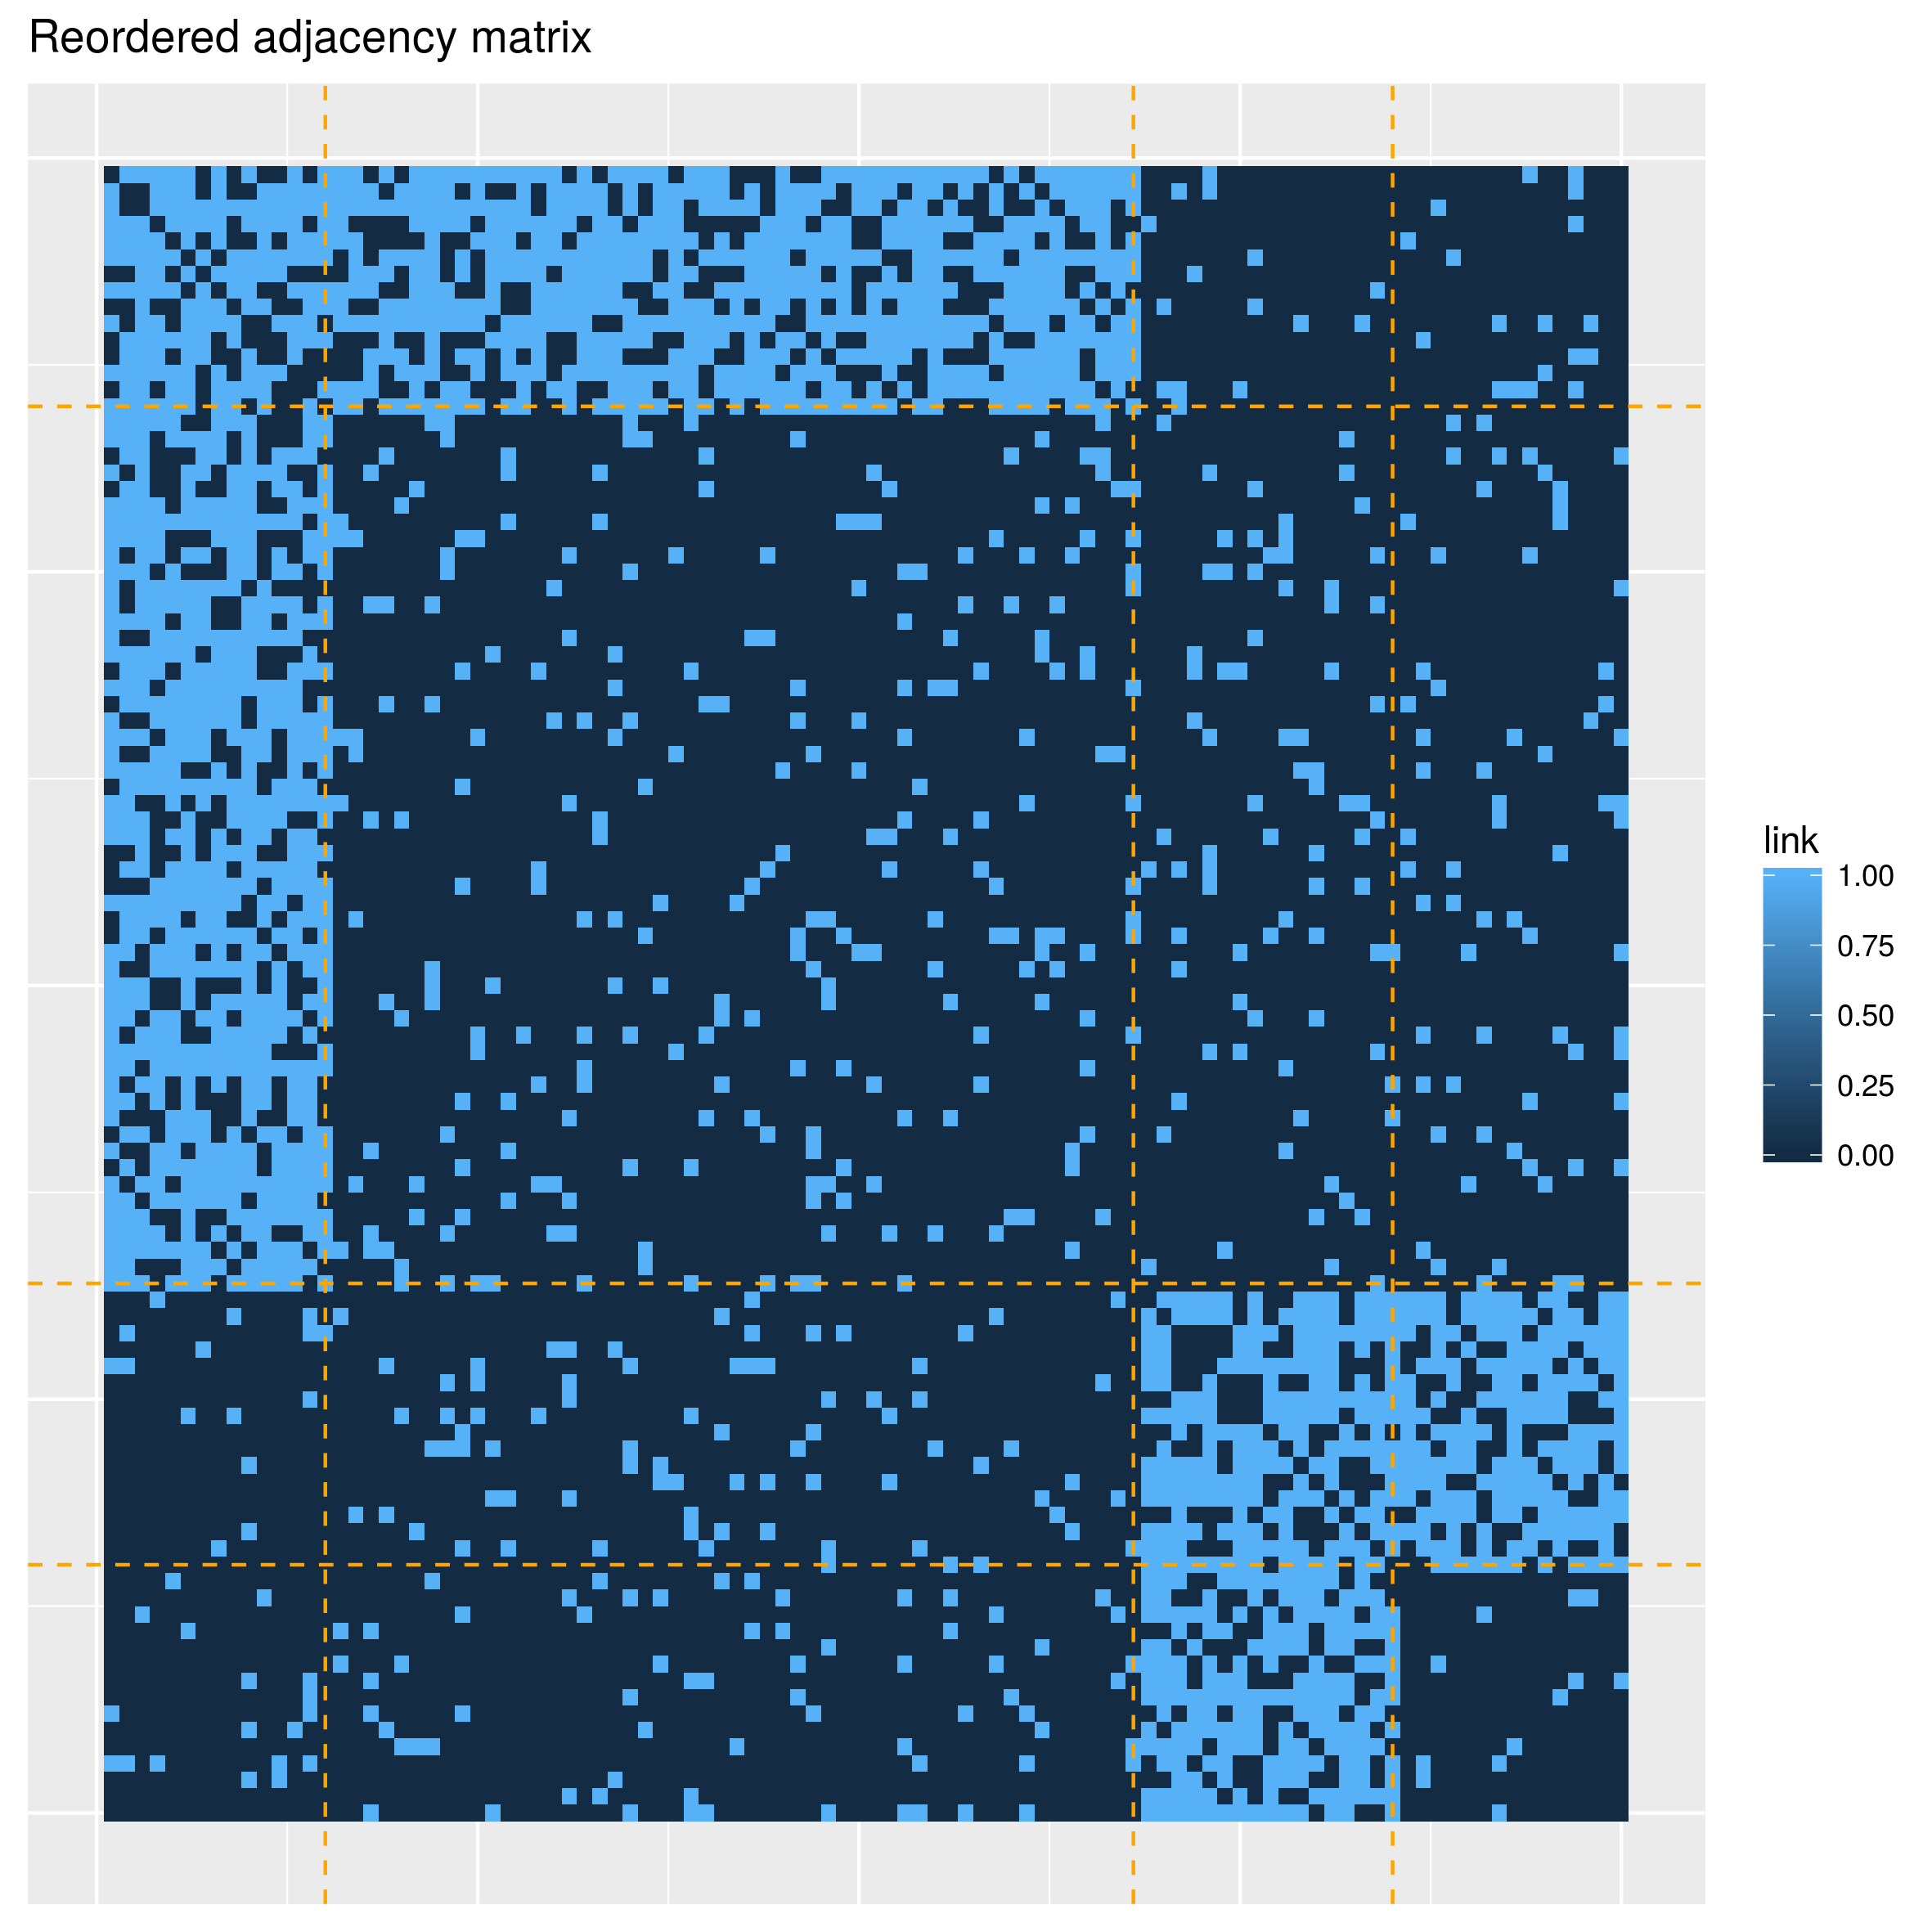
\includegraphics[scale=.2]{plots/Etoile_reordered_adja_with_groups.png}&
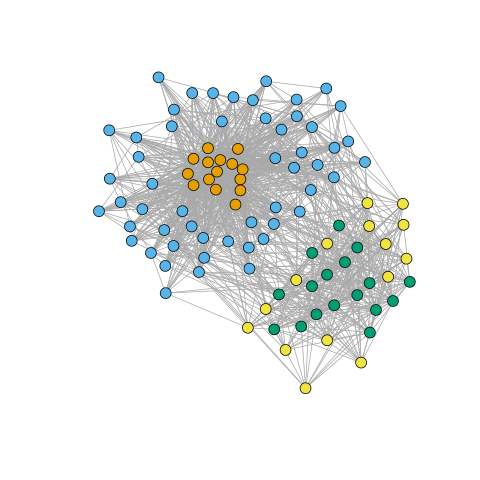
\includegraphics[scale=.2]{plots/Etoile_graphe_with_colors.png}&
   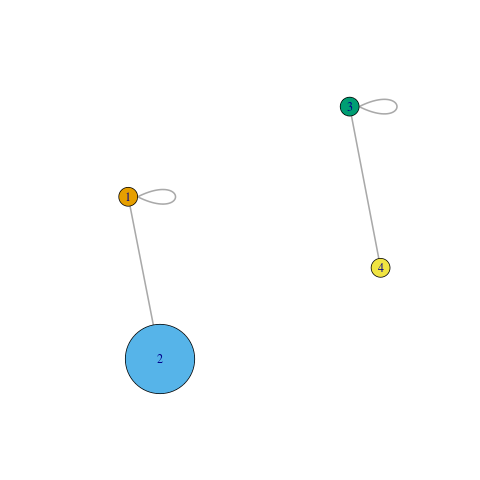
\includegraphics[scale=.2]{plots/Etoile_graphe_resume.png}
 \end{tabular}

\begin{tabular}{cc}
    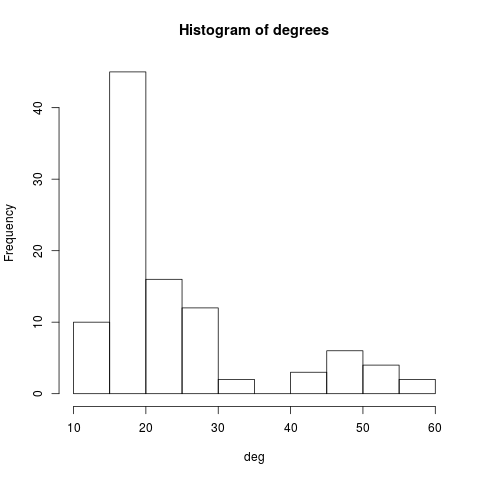
\includegraphics[scale=.2]{plots/Etoile_histogram_degree.png}&
   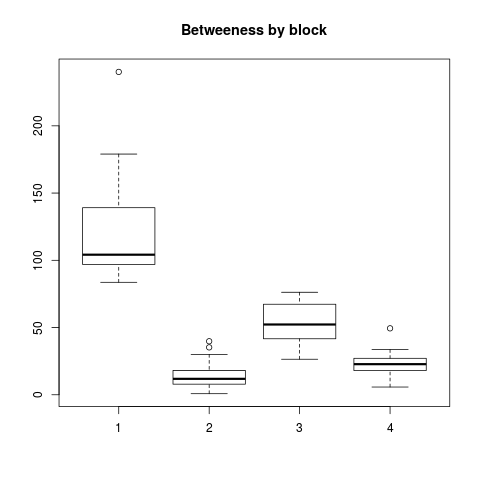
\includegraphics[scale=.2]{plots/Etoile_betweeness.png}
 \end{tabular}

\end{frame}



%-------------------------------------------------------------------------------------
\begin{frame}
\frametitle{Community network  generated by SBM}

\centering
\begin{tabular}{cc}
 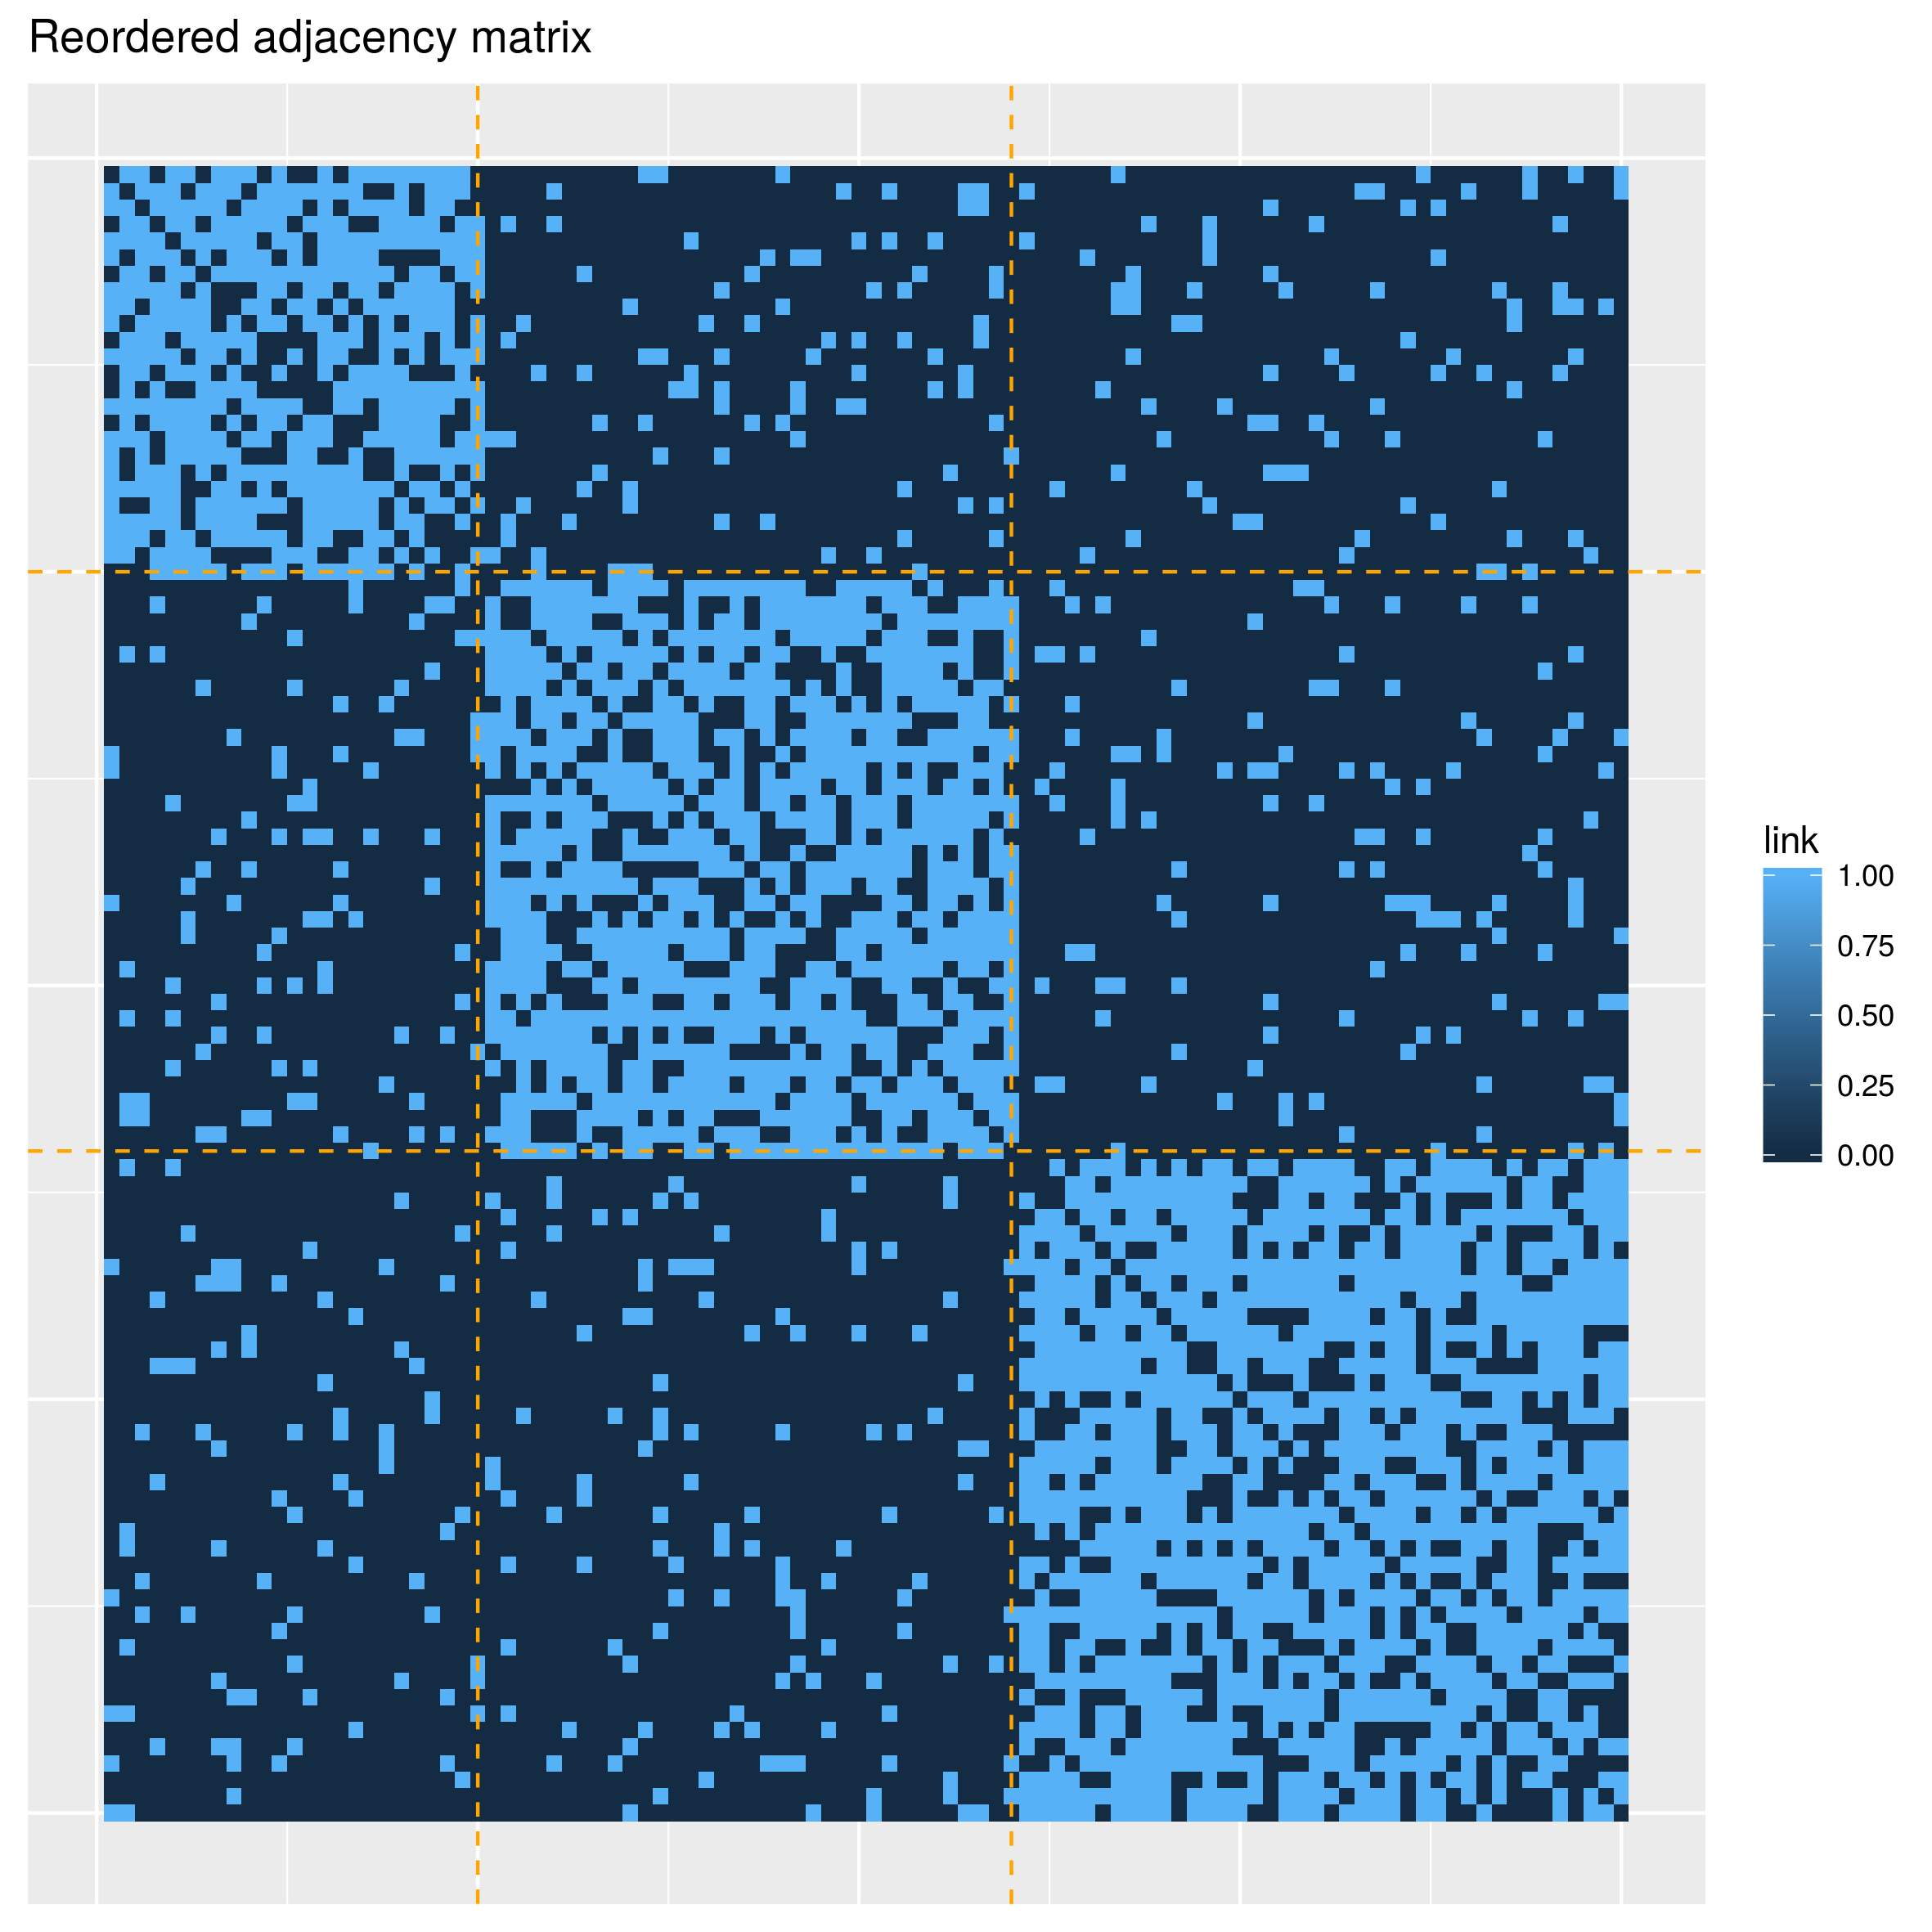
\includegraphics[scale=.2]{plots/Affiliation_reordered_adja_with_groups.png}&
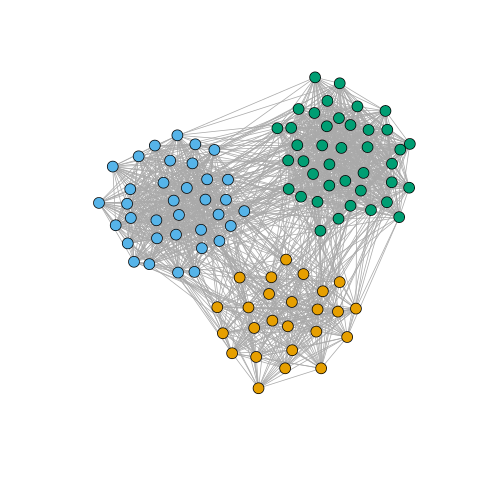
\includegraphics[scale=.2]{plots/Affiliation_graphe_with_colors.png} 
 \end{tabular}

\begin{tabular}{cc}
   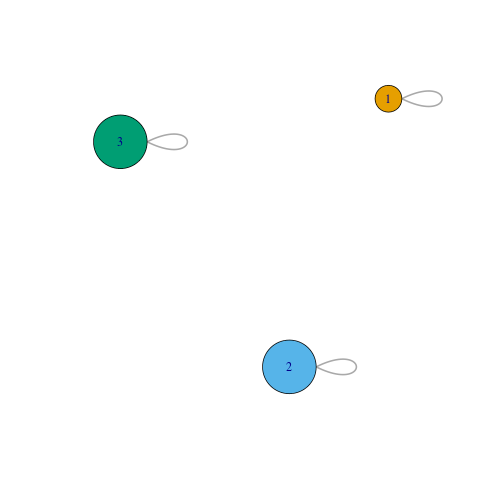
\includegraphics[scale=.2]{plots/Affiliation_graphe_resume.png}
    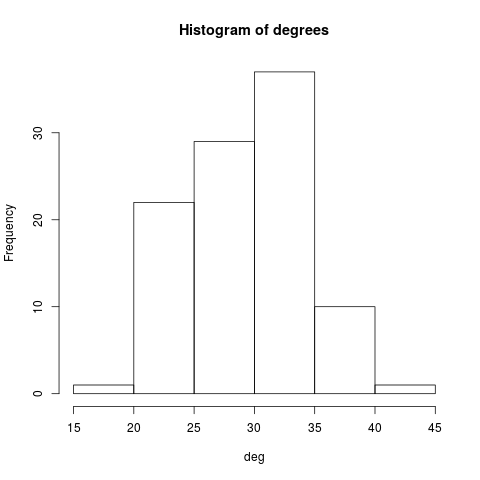
\includegraphics[scale=.2]{plots/Affiliation_histogram_degree.png}&
 \end{tabular}

\end{frame}


%-------------------------------------------------------------------------------------
\begin{frame}
\frametitle{Nestedness  generated by SBM}

\centering
\begin{tabular}{cc}
 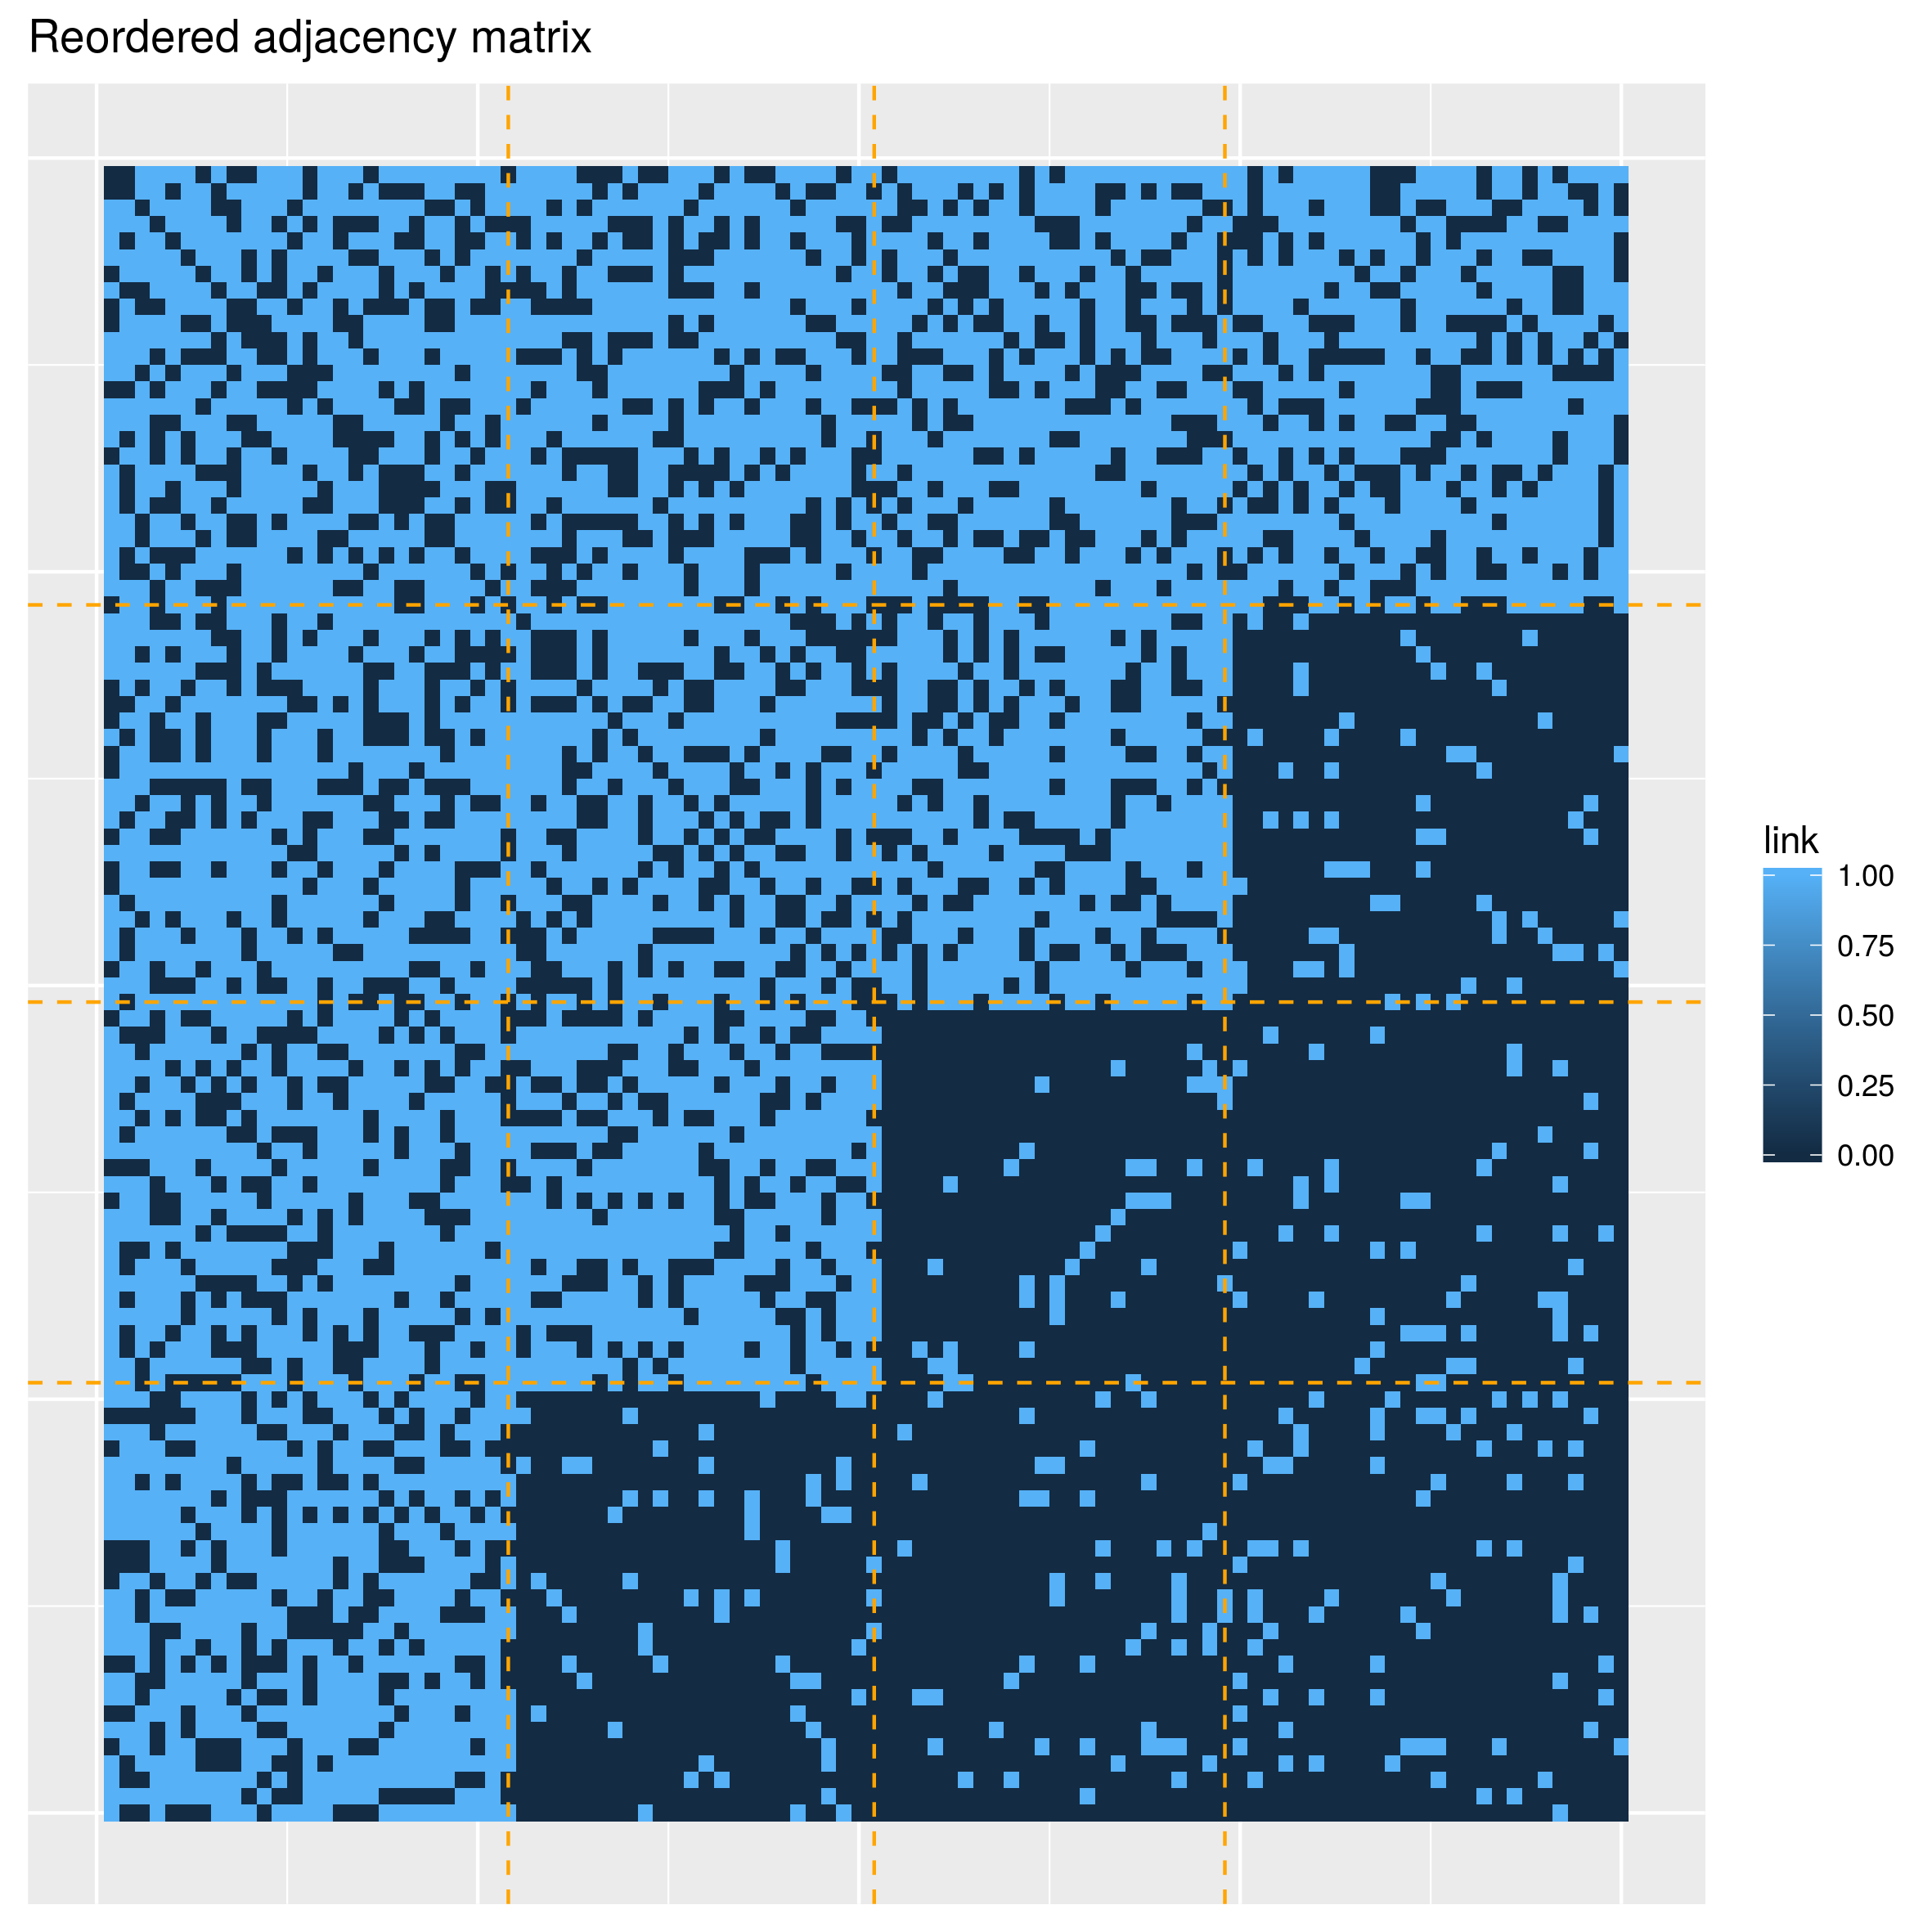
\includegraphics[scale=.2]{plots/Nested_reordered_adja_with_groups.png}&
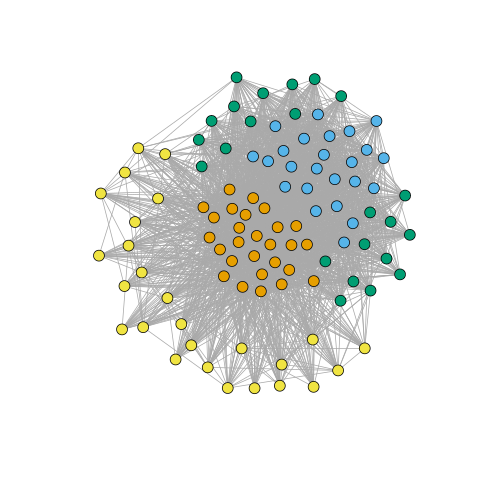
\includegraphics[scale=.2]{plots/Nested_graphe_with_colors.png} 
 \end{tabular}

\begin{tabular}{cc}
   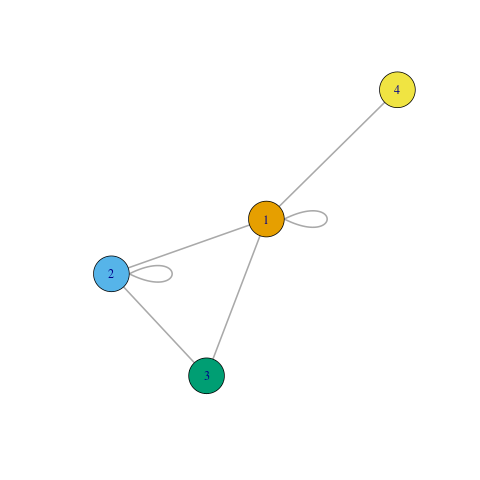
\includegraphics[scale=.2]{plots/Nested_graphe_resume.png}
    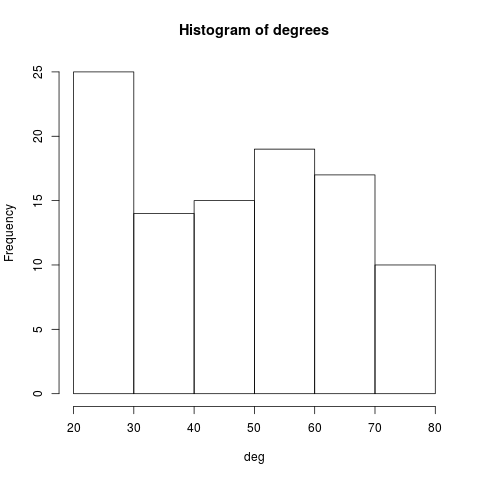
\includegraphics[scale=.2]{plots/Nested_histogram_degree.png}&
 \end{tabular}

\end{frame}

%----------------------------------------------------------------

%----------------------------------------------------------------

 
 

\begin{frame}
  \frametitle{Inférence statistique}
 
    \begin{center}
  \begin{overlayarea}{\textwidth}{.5\textheight}
      \begin{columns}
        \begin{column}{.45\paperwidth}
        \begin{tikzpicture}
          %% UN GRAPH

          \tikzstyle{every edge}=[-,>=stealth',shorten >=1pt,auto,thin,draw]
          \tikzstyle{every state}=[draw=none,text=white,scale=0.65, font=\scriptsize, transform shape]
          \tikzstyle{every node}=[fill=lightgray]
          % premier cluster
          \node[state] (A1) at (0,0.5) {N1};
          \node[state] (A2) at (1,0.5) {N2};
          \node[state] (A3) at (.5,1.5) {N3};

          \path (A2) edge [bend left] node[fill=white,below=.1cm]
          {}
          (A1)
          (A1) edge [bend left] (A3)
          (A3) edge [bend left] (A2);

          \tikzstyle{every node}=[fill=blue!80!black]
          \foreach \angle/\text in {234/N1, 162/N2, 90/N3, 18/N4, -54/N5} {
            \node[fill=lightgray,state,xshift=5cm,yshift=3.5cm]     (\text)    at
            (\angle:1cm) {\text};
          }
          \path (B2) edge (B5)
          (B1) edge (B4);
          \foreach \from/\to in {1/2,2/3,4/5,5/1}{
            \path (B\from) edge [bend left] (B\to);
          }

          \path    (B3)    edge     [bend    left]    node[fill=white]
          {}  (B4) ;
          
          \tikzstyle{every node}=[fill=lightgray]
          % troisime cluster
          \node[state] (C1) at (3,-.5) {N1};
          \node[state] (C2) at (4,0) {N2};

          \path (C1) edge [bend right] (C2);

          % inter cluster
          \path (A3) edge [bend right]  (B2)
          (A3)    edge    [bend    left]    node[fill=white]
          {}
          (B3)
          (C2) edge [bend right] node[fill=white,right]
          {}
          (B4)
          (A2) edge [bend right] node[fill=white]
          {}
          (C1);
        \end{tikzpicture}
        \end{column}
        \begin{column}{.5\paperwidth}
          \begin{small}
            \begin{block}{Inférence}
             
              \begin{itemize}
              \item
                $\mathcal{K}=\{\textcolor{yellow!40!orange}{\bullet},\textcolor{blue!80!black}{\bullet},\textcolor{green!50!black}{\bullet}\}$,
                $\text{card}(\mathcal{K})$ known
             \begin{itemize}
             
              \item  $\pi_\bullet  =  ?$,
              \item      $\alpha_{\textcolor{yellow!40!orange}{\bullet}\textcolor{blue!80!black}{\bullet}}     =      ?$
\item $Z_1, \dots, Z_n  = ? $
\end{itemize}

\item $\text{card}(\mathcal{K})$?
              \end{itemize}
            \end{block}
          \end{small}
        \end{column}
      \end{columns}
    \end{overlayarea}
    \end{center}
    \medskip

    
    \textcolor{blue}{Nowicki, \& Snijders (2001), Daudin et al. (2008)}
    
    \bigskip
    
\textcolor{blue}{R package: blockmodels.}
%     
%     \begin{thebibliography}{99}
%       \begin{scriptsize}
%       \bibitem[NS]{NS} Nowicki, Snijders, JASA, 2001 \newblock Estimation and prediction for
%         stochastic   blockstructures.
%         \textcolor{black}{} 
%       \bibitem[DRP]{DRP}   Daudin,  Picard,   Robin,  Statistics   and
%         Computing, 2008 \newblock A mixture model for random graphs. 
%       \end{scriptsize}
%   \end{thebibliography}

\end{frame}
%----------------------------------------------------------------


\begin{frame}{Exemple du Vanuatu}
 
\begin{overlayarea}{10cm}{20cm}


\only<2>{ \begin{tabular}{cc} 
  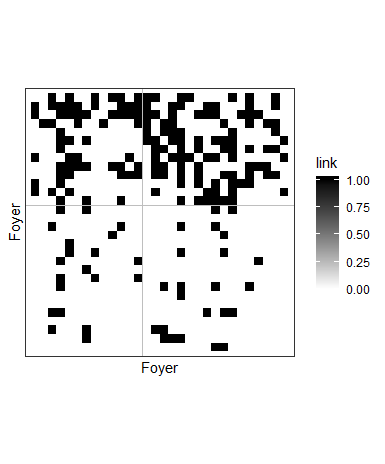
\includegraphics[width = 5cm]{plots/Vanuatu_estimmatrix.png} &
 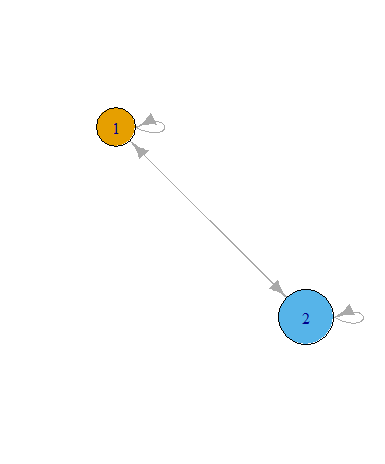
\includegraphics[width = 5cm]{plots/Vanuatu_graphestim.png}
\end{tabular}
}


\only<1>{ \begin{tabular}{cc}
  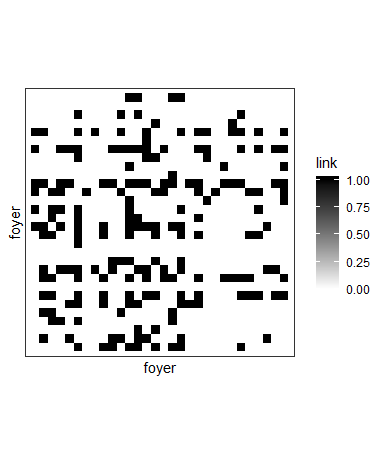
\includegraphics[width = 5cm]{plots/Vanuatu_matrix.png} &
 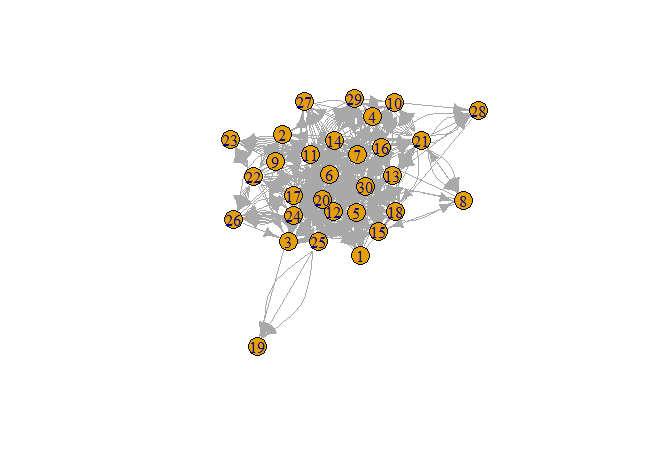
\includegraphics[width = 5cm]{plots/Vanuatu_directed.png}
\end{tabular}}
\end{overlayarea}


\end{frame}





%-------------------------------------------------------------------------------------

\section{Latent block model (LBM)}
%reseau interaction qcq

\begin{frame}{Probabilistic model for binary  bipartite networks}

Let $Y_{ij}$ be a bi-partite network. Individuals in row and cols are not the same. 

\begin{block}{Latent variables : bi-clustering}
\begin{itemize}
\item Nodes $i= 1,\dots,n_1$   partitionned into $K_1$ clusters,  nodes $j= 1,\dots,n_2$  partitionned into $K_2$ clusters
\item $$\begin{array}{cl}
Z^1_i = k & \mbox{if node $i$ belongs to cluster (block) $k$}\\
Z^2_j = \ell & \mbox{if node $j$ belongs to cluster (block) $\ell$}
\end{array}$$
\item $Z^1_i, Z^2_j$ independent variables
$$ \mathbb{P}(Z^1_i = k) = \pi^1_k,\quad  \mathbb{P}(Z^2_j = \ell) = \pi^2_\ell$$
\end{itemize}
\end{block}

\end{frame}

%-------------------------------------------------------------------------------------

\begin{frame}{Probabilistic model for binary  bipartite networks}


\begin{block}{Conditionally to $(Z^1_i)_{i=1,\dots,n_1},(Z^2_j)_{j=1,\dots,n_2}$... }

$(Y_{ij})$ independent and 
\begin{eqnarray*}
 Y_{ij}  | Z^1_i, Z^2_j \sim  \mathcal{B}ern(\alpha_{Z^1_i,Z^2_j}) \quad \Leftrightarrow \quad   \mathbb{P}(Y_{ij} = 1 | Z^1_i = k, Z^2_j = \ell)  =  \alpha_{k\ell}
\end{eqnarray*}
\end{block}
 

\textcolor{blue}{Govaert \& Nadif (2008)}  


\end{frame}

%-------------------------------------------------------------------------------------


\begin{frame}
\frametitle{Latent Block Model : illustration}

 \begin{center}
    \begin{overlayarea}{\textwidth}{.5\textheight}
      \begin{columns}
        \begin{column}{.45\paperwidth}
        \centering
        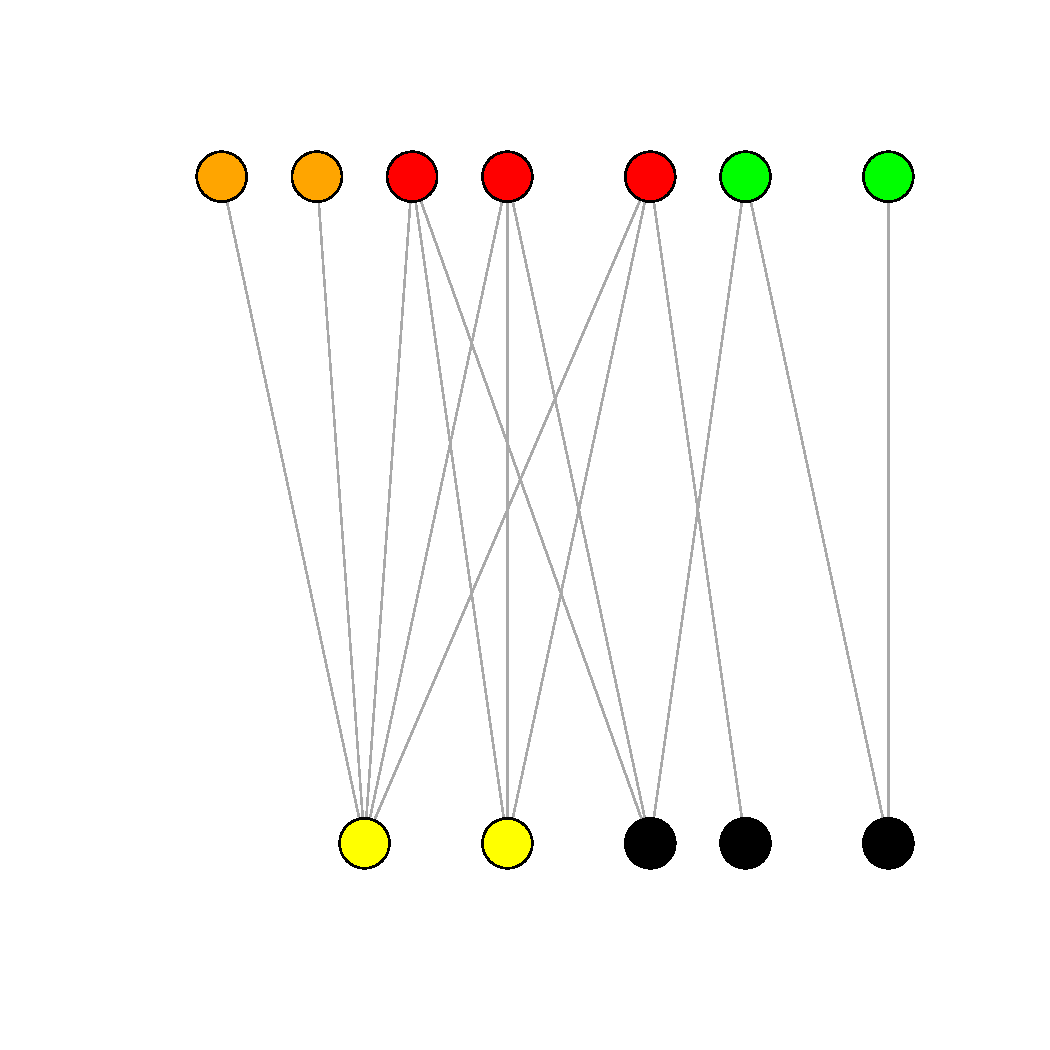
\includegraphics[scale=.3]{plots/LBM_exemple.pdf}
        \end{column}
        \begin{column}{.5\paperwidth}
          \begin{small}
            \begin{block}{Latent Block Model}
              \begin{itemize}
              \item
                $n_1$ row nodes $\mathcal{K}_1=\{\textcolor{red}{\bullet},\textcolor{orange}{\bullet},\textcolor{green}{\bullet}\}$
                classes
              \item  $\pi^1_\bullet  =  \mathbb{P}(i  \in  \bullet)$,
                $\bullet\in\mathcal{K}_1,i=1,\dots,n$
              \item $n_2$ column nodes $\mathcal{K}_2=\{\textcolor{yellow}{\bullet},\textcolor{black}{\bullet}\}$
                classes
               \item  $\pi^2_\bullet  =  \mathbb{P}(j  \in  \bullet)$,
                $\bullet\in\mathcal{K}_2,j=1,\dots,m$
              \item      $\alpha_{\textcolor{red}{\bullet}\textcolor{yellow}{\bullet}}     =      \mathbb{P}(i
                \leftrightarrow j | i\in\textcolor{red}{\bullet},j\in\textcolor{yellow}{\bullet})$
              \end{itemize}
            \end{block}
          \end{small}
        \end{column}
      \end{columns}
    \end{overlayarea}
  \end{center}
  
%\begin{eqnarray*}
%&(Z_i) &  \ \sim^{\text{iid}} \mathcal{M}(1,\alpha) \ \text{et} \  Z_{i} \in \{1,...,Q\}, \\ 
% &(Y_{ij})&| \ \{Z_{i},Z_{j}\} \sim^{\text{ind}} \mathcal{B}(\pi_{Z_{i}Z_{j}}).\\
%\end{eqnarray*}

% Proposition Julien
\begin{align*}
Z^1_i = \mathbf{1}_{\{i \in \bullet\}}  \ & \sim^{\text{iid}} \mathcal{M}(1,\bpi^1), \quad \forall\bullet \in \mathcal{Q}_1, \\ 
Z^2_j=\mathbf{1}_{\{j \in \bullet\}}  \ & \sim^{\text{iid}} \mathcal{M}(1,\bpi^2), \quad \forall\bullet \in \mathcal{Q}_2, \\
Y_{ij} \ | \ \{i\in\textcolor{red}{\bullet},j\in\textcolor{yellow}{\bullet}\}
& \sim^{\text{ind}} \mathcal{B}ern(\alpha_{\textcolor{red}{\bullet}\textcolor{yellow}{\bullet}})\\
\end{align*}


\textcolor{blue}{Govaert \& Nadif (2008)} and 
\textcolor{blue}{R package: blockmodels} as well.

\end{frame}





%---------------------------------------------------------------------------


\begin{frame}
 \frametitle{Valued-edge networks}
 

\begin{block}{Values-edges networks}
 Information on edges can be something different from presence/absence.
 It can be:
 \begin{enumerate}
  \item a count of the number of observed interactions,
  \item a quantity interpreted as the interaction strength,
  \end{enumerate}

 \end{block}

 \bigskip
 
 


\begin{block}{ Natural extensions of SBM and LBM}
 \begin{enumerate}
  \item Poisson distribution: $Y_{ij} \ | \ \{i\in\textcolor{yellow!40!orange}{\bullet},j\in\textcolor{blue!80!black}{\bullet}\}
\sim^{\text{ind}} \mathcal{P}(\lambda_{\textcolor{yellow!40!orange}{\bullet}\textcolor{blue!80!black}{\bullet}})$,
 \item Gaussian distribution: $Y_{ij} \ | \ \{i\in\textcolor{yellow!40!orange}{\bullet},j\in\textcolor{blue!80!black}{\bullet}\}
\sim^{\text{ind}} \mathcal{N}(\mu_{\textcolor{yellow!40!orange}{\bullet}\textcolor{blue!80!black}{\bullet}},\sigma^2)$,
\textcolor{blue}{Mariadassou et al. (2010)}
\item More generally, 
  $$Y_{ij} \ | \ \{i\in\textcolor{yellow!40!orange}{\bullet},j\in\textcolor{blue!80!black}{\bullet}\}
\sim^{\text{ind}} \mathcal{F}(\theta_{\textcolor{yellow!40!orange}{\bullet}\textcolor{blue!80!black}{\bullet}})$$
 \end{enumerate}
 \end{block}
 \bigskip

\end{frame}



%---------------------------------------------------------------------- 


\begin{frame}{Exemple sur Vanuatu Foyers/espèces cultivées}

 \begin{tabular}{cc}
\end{tabular}


\begin{overlayarea}{10cm}{20cm}
\only<1>{ \begin{tabular}{cc}
  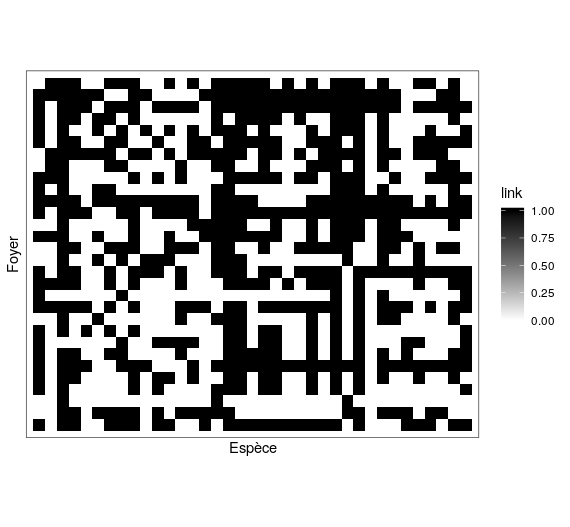
\includegraphics[width = 5cm]{plots/Vanuatu_incidence.png} &
 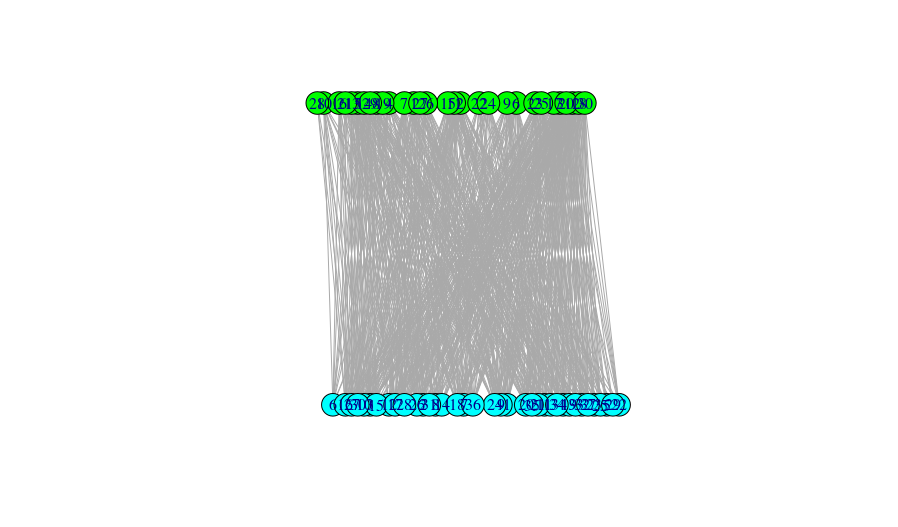
\includegraphics[width = 8cm]{plots/Vanuatu_bipartite.png}
\end{tabular}}

\only<2>{ \begin{tabular}{cc} 
  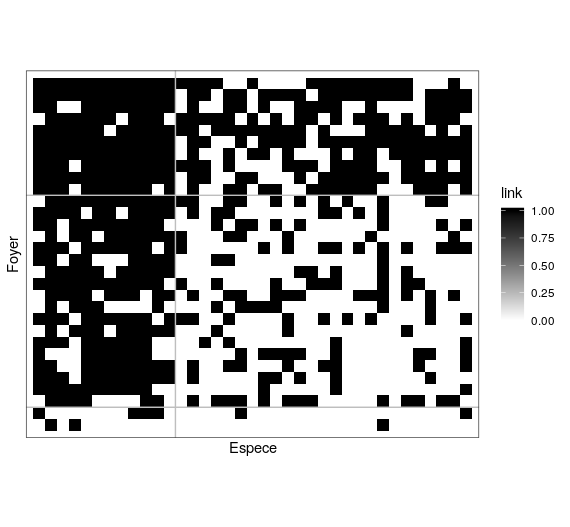
\includegraphics[width = 5cm]{plots/Vanuatu_incidenceestim.png} &
 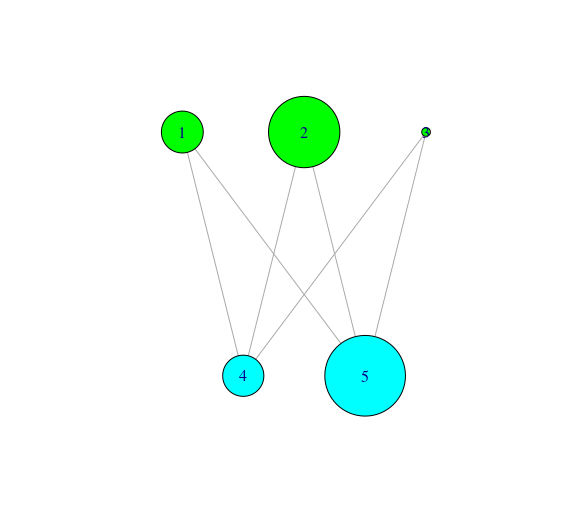
\includegraphics[width = 8cm]{plots/Vanuatu_bipartiteestim.png}
\end{tabular}
}

\end{overlayarea}





\end{frame}

\end{document}
%---------------------------------------------------------------------------------


  
  


%%%Local Variables:
%%% mode: latex
%%% eval: (TeX-PDF-mode 1)
%%% ispell-local-dictionary: "francais"
%%% eval: (flyspell-mode 1)
%%%End:


